\chapter[Deseño]{
  \label{chp:disenho}
  Deseño
}
\minitoc
\newpage


\section{Modelo de datos}

Á hora de definir esta cuestión, tratáronse de respectar as regras do modelo relacional de bases de datos, porén, fixeronse algunhas excepcións motivadas por esixencia da elección do framework Django:

\begin{itemize}
	\item Claves primarias subrogadas: Django encárgase da identificación das tuplas engadindo ás táboas un campo numérico enteiro de incremento automático. Isto utilizarase en todas as táboas sen excepción.
	
	\item Relación 1-1: Como se ve no diagrama Entidade-Relación da figura \ref{fig:diagrama_er}, existe unha relación 1-1 entre a entidade User e a súa entidade feble UserProfile. O motivo da existencia desta última é que se decidiu utilizar a entidade de usuario nativa de Django, co cal fíxose necesaria unha nova táboa para cubrir os atributos de usuario necesarios especificamente para o proxecto. 
\end{itemize}

No diagrama Entidade-Relación da figura \ref{fig:diagrama_er} pódense ver as táboas empregadas sen incluir aquelas automáticamente xeradas para o correcto funcionamento de Django e Celery a excepción da xa mencionada User. Por motivos de claridade, non se incluíron os atributos agás aqueles adicionais nas táboas correspondentes ás relacións \say{N a N}.

A estrutura da BD tradúcese na aplicación ás clases definidas no paquete models.py que se ve na figura \ref{fig:clase_models}. Por claridade, nese diagrama de clases só se incluíron os atributos máis representativos ou explicativos das relacións entre clases.

\begin{figure}[h]
	\centering
	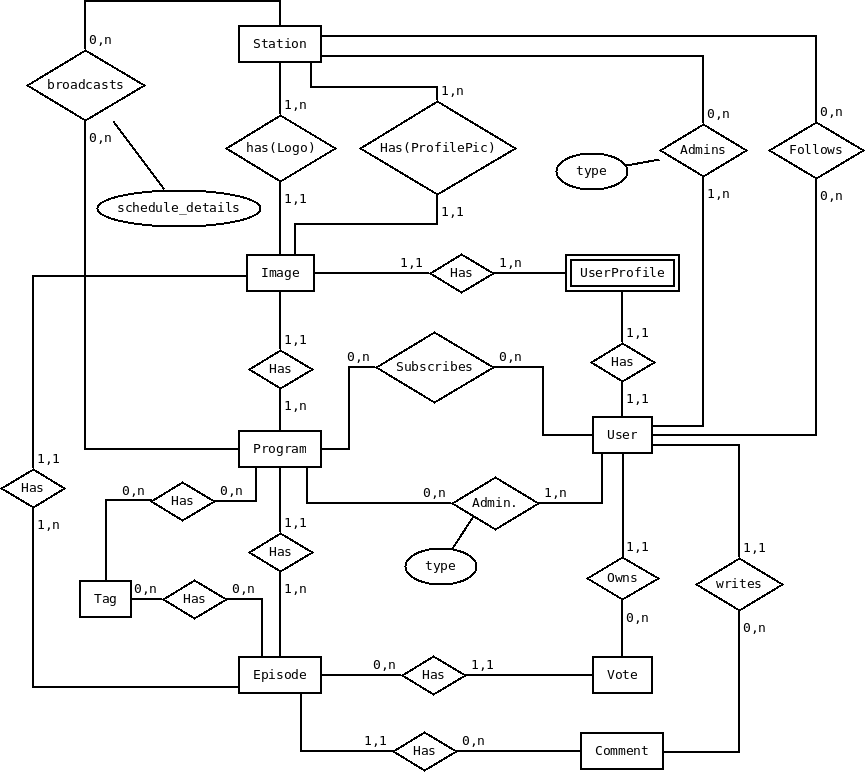
\includegraphics[scale=0.5,keepaspectratio=true]{./images/ER_diagrama.png}
	\caption{Diagrama Entidade-Relación da Base de Datos.}
	\label{fig:diagrama_er}
\end{figure}

\begin{figure}[h]
	\centering
	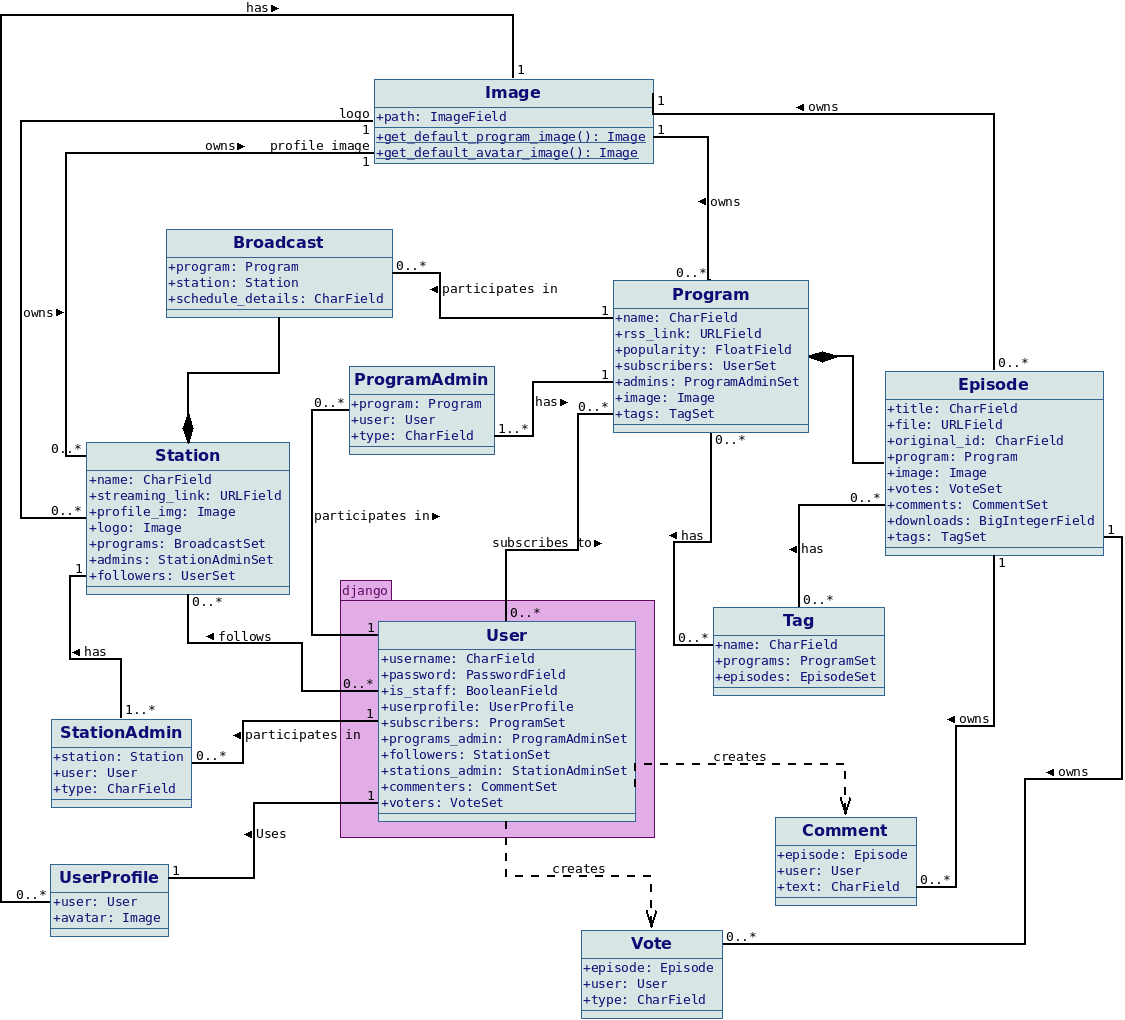
\includegraphics[scale=0.4,keepaspectratio=true]{./images/class_diagram.png}
	\caption{Diagrama de clases do paquete models.}
	\label{fig:clase_models}
\end{figure}


\begin{figure}[h]
	\centering
	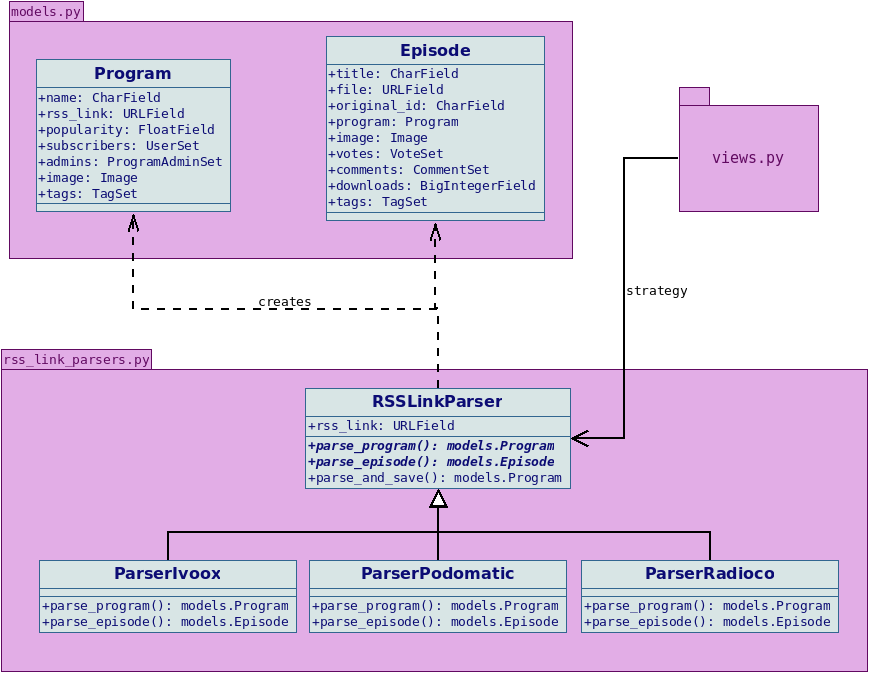
\includegraphics[scale=0.5,keepaspectratio=true]{./images/strategy.png}
	\caption{Patrón Estratexia utilizado para o procesamento de RSS.}
	\label{fig:strategy}
\end{figure}


\subsection{Os usuarios}

Os usuarios están definidos por dúas táboas: User e UserProfile que se corresponden coas clases User, do paquete django.contrib.auth.models, e UserProfile, definida polo desenvolvedor e, polo tanto, includida no paquete models.py. Esta segunda considerámola coma feble de User pois a existencia dun perfil está vencellada de xeito ineludible á existencia dun usuario.




